\section{Methods used}


\subsection{Central truncation}

\begin{frame}{Central Truncation}

	\begin{itemize}
		\item The most common and straightforward approach used in practice to handle
		texts exceeding the context size.
		\item Generally, sequences are truncated from the end before processing.
		\item Some studies show that truncating the middle produced better results
		\citep{sun2019fine, worsham-kalita-2018-genre}.
		\item We keept a fraction of the tokens from the head and the tail, i.e. truncated
		the middle.
		\item Hyperparameter $head\_size \in [0, 1]$ controls the fraction of tokens taken
		from the head.
	\end{itemize}

	% \item This pipeline is based on Central Truncation, i.e. truncating
	% tokens from the middle of the text.
	% \item<2-> Hyperparameter $head\_size \in [0, 1]$: Controls the fraction
	% of tokens taken from the head.
	% \item<3-> $head\_size = 0$ means all tokens are taken from the tail, and
	% $head\_size = 1$ means all tokens are taken from the head.
	% \item<4-> Tokens from the head and the tail are concatenated and sent to the summarizer.


\subsection{Document Skimming}

\begin{frame}{Document Skimming}

	\begin{itemize}
		\item This approach is inspired by the fast reading technique "skimming".
		\item<2-> It involves reading while skipping some parts of the text for efficiency.
		\item<3> Reader attempts to skip the redundant or irrelevant parts.
	\end{itemize}

	\only<1>{
		\vskip 3.4cm
	}

	\only<2->{
		\vskip .5cm
		\begin{figure}
			\centering
			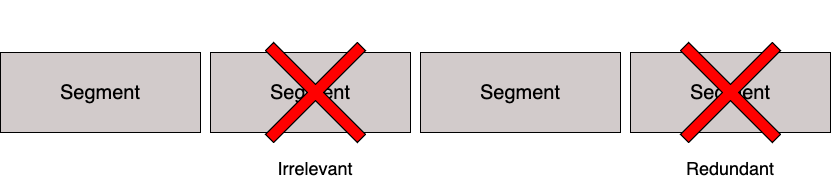
\includegraphics[width=\textwidth]{Images/skim.png}
		\end{figure}
	}

\end{frame}

\begin{frame}{Document Skimming (Contd.)}

	\begin{itemize}
		\item This method involves uniformly sampling the text segments to fill the LLM's
		context size.
		\item<3-> This ensures we capture details from every part of the text.
		\item<4> A similar approach is taken by \citet{wang2024videoagent} to develop
		VideoAgent for QA on long videos.
	\end{itemize}

	\only<1>{
		\vskip 3.81cm
	}

	\only<2->{
		\vskip 1cm
		\begin{figure}
			\centering
			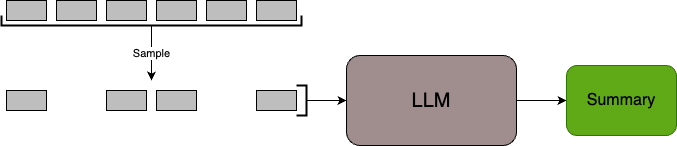
\includegraphics[width=1\textwidth]{Images/doc-skim.png}
		\end{figure}
}

\end{frame}


\subsection{Skimming w/ Extraction}

\begin{frame}{Document Skimming with Keyword Extraction}

	\begin{itemize}
		\item Instead of randomly sampling the text segments, we can make use of important
		keywords or phrases from the text for sampling.
		\item<2-> This can be achieved by using extractive summarization algorithms that can
		efficiently handle very long texts.
		\item<3-> We can then compute a probability distribution for the segments using
		similarity scores.
		\item<4> We will be experimenting with: TextRank, LexRank, PacSum, Luhn's algorithm,
		and SummaRuNNer.
	\end{itemize}

\end{frame}


% \subsection{Using Convolutions}

% \begin{frame}{Summarizing using Convolutions!}

% 	\begin{itemize}
% 		\item This approach starts by segmenting the text and encoding the segments.
% 		\item<2-> Since the segments will be short, we can use a small encoder to efficiently
% 		encode the them.
% 		\item<3-> We will then use 1D convolutions as an efficient substitute to the
% 		quadratic self attention!
% 		\item<4-> A similar methodolody is applied by \citet{chen2022long} to classify long
% 		Chinese news.
% 		\item<5> Longformer \citep{beltagy2020longformer} uses windowed self attention to
% 		reduce the complexity, but ours is cheaper.
% 	\end{itemize}
	
% \end{frame}


\subsection{Pipeline 2}

\begin{frame}{Pipeline 2}
	
	\begin{itemize}
		\item This pipeline is based on \textbf{Document Skimming}, i.e. skipping over some parts
		of the document.
		\item<2-> We start by segmenting the text into chunks of sentences.
		\item<3-> The size of a segment is decided by number of words in it.
		\item<4-> Each segment must have at least $min\_words$ words, which is a
		hyperparameter.
	\end{itemize}

\end{frame}

\begin{frame}{Pipeline 2 (contd.)}
	
	\begin{itemize}
		\item We then uniformly sample the segmented text to fill the context size.
		\item<2-> Each segment has a probability $p$ of being selected.
		\item<3-> $ p = context\_size / total\_tokens $
		(derivation provided in report)
		\item<4-> The selected segments are then concatenated with segment delimiters
		and sent to the summarizer.
	\end{itemize}

\end{frame}


\subsection{Pipeline 3}

\begin{frame}{Pipeline 3}

	\begin{itemize}
		\item This pipeline is also based on \textbf{Document Skimming} and is a modification
		of \textbf{Pipeline 2}.
		\item<2-> After sampling the segments, segments similar to previously picked
		segments are removed.
		\item<3-> This is done by comparing the segment embeddings generated by
		a sentence transformer from Hugging Face.
		\item<4-> We linearly traverse the sampled segments and track the mean of the
		sentence embeddings.
		\item<5> Hyperparameter $threshold \in (0, 1]$: Segment $i$ is removed if
		\[ \mathrm{cos\_sim}(mean\_emb, emb_i) \ge threshold \]
	\end{itemize}

\end{frame}


\subsection{Pipeline 4}

\begin{frame}{Pipeline 4}

	\begin{itemize}
		\item This pipeline is also a modification of \textbf{Pipeline 2} and is similar to
		\textbf{Pipeline 3}.
		\item<2-> Instead of removing similar segments after sampling, we first remove similar
		segments and then uniformly sample the segments.
		\item<3-> Although this pipeline might be slower than \textbf{Pipeline 3}, it ensures
		better utilization of the LLM's context size.
	\end{itemize}
	
\end{frame}
